
\documentclass[10pt]{beamer}
\usetheme{metropolis}

% ── Packages ──
\usepackage{amsmath,amssymb,amsthm}
\usepackage{tikz}
\usetikzlibrary{positioning,arrows.meta,fit,matrix,backgrounds,calc,shapes.geometric,decorations.pathreplacing}
\usepackage{graphicx}
\usepackage{array}
\usepackage{etoolbox}
\usepackage{cancel}

% ── Theorem environments ──
\theoremstyle{definition}
\newtheorem{defi}{Definition}[section]
\newtheorem{prop}{Proposition}[section]
\newtheorem{thm}{Theorem}[section]
\newtheorem{cor}{Corollary}[section]

% Custom theorem styles with colors
\setbeamercolor{block title}{bg=red!75!black,fg=white}
\setbeamercolor{block body}{bg=yellow!10!white}

\AtBeginEnvironment{prop}{%
  \setbeamercolor{block title}{bg=yellow!75!black,fg=black}%
  \setbeamercolor{block body}{bg=yellow!10!white}%
}
\AtEndEnvironment{prop}{%
  \setbeamercolor{block title}{bg=red!75!black,fg=white}%
}

\AtBeginEnvironment{thm}{%
  \setbeamercolor{block title}{bg=yellow!75!black,fg=black}%
  \setbeamercolor{block body}{bg=yellow!10!white}%
}
\AtEndEnvironment{thm}{%
  \setbeamercolor{block title}{bg=red!75!black,fg=white}%
}

\AtBeginEnvironment{cor}{%
  \setbeamercolor{block title}{bg=yellow!75!black,fg=black}%
  \setbeamercolor{block body}{bg=yellow!10!white}%
}
\AtEndEnvironment{cor}{%
  \setbeamercolor{block title}{bg=red!75!black,fg=white}%
}

% ── Highlighting ──
\newcommand{\x}[1]{\alert{\textbf{#1}}}

% ── Color shortcuts ──
\newcommand{\rd}[1]{{\color{red!70!black}#1}}
\newcommand{\bl}[1]{{\color{blue!70!black}#1}}
\newcommand{\gn}[1]{{\color{green!60!black}#1}}

\title{Lecture 18: The Exponential Function}
\subtitle{MATH203 Applied Linear Algebra}
\date{}
\titlegraphic{}

\begin{document}
\maketitle


% ┌─────────────────────────────────────────────────────────────────────┐
% │ SECTION 1: WHAT IS e? — COMPOUND INTEREST                         │
% │                                                                    │
% │ THE MACRO DESIGN: START FROM A NAIVE QUESTION                     │
% │                                                                    │
% │ The audience enters knowing complex numbers from L17. The          │
% │ exponential was previewed: "What does e^{iθ} mean?" Now we        │
% │ answer by going back to the very beginning: what IS e?            │
% │                                                                    │
% │ The compound interest story makes the LIMIT definition feel        │
% │ inevitable. It's not a formula handed from above — it's the        │
% │ answer to "what happens when you compound more and more often?"   │
% │                                                                    │
% │ Emotional arc: curiosity → surprise (it doesn't blow up) →        │
% │ satisfaction (it converges to a specific number).                   │
% └─────────────────────────────────────────────────────────────────────┘
\section{What Is $e$?}


\begin{frame}[shrink=5]{A Question About Money}

You deposit \$1 in a bank. The bank's rule: \x{100\% interest per year}, computed \x{linearly}.

\vfill

\begin{itemize}
\item After 1 year: $\$1 + 100\% = \$2$
\item After 2 years: $\$1 + 200\% = \$3$
\item After half a year: $\$1 + 50\% = \$1.50$
\end{itemize}

\vfill\pause

\textbf{Someone discovers a trick:} Withdraw after 1 year (\$2), immediately re-deposit.

Now the second year's interest is computed on \$2, not \$1:
$$\text{After 2 years} = \$2 + 100\% \times \$2 = \$4 \quad \text{(instead of \$3!)}$$

\vfill\pause

\textbf{Better trick:} Withdraw after \x{half} a year (\$1.50), re-deposit.

$$\text{After 1 year} = \$1.50 + 50\% \times \$1.50 = \$2.25 \quad \text{(instead of \$2!)}$$

\end{frame}


\begin{frame}[shrink=5]{The Greedy Strategy}

\textbf{Idea:} Withdraw and re-deposit as \x{frequently as possible}.

\vfill

Every $\frac{1}{n}$ of a year, take out your money and put it back:

$$\text{After each period:} \quad \text{balance} \times \left(1 + \frac{1}{n}\right)$$

After $n$ periods (one full year):

$$\text{Final balance} = \$1 \times \left(1 + \frac{1}{n}\right)^n$$

\vfill\pause

\textbf{Question:} As $n \to \infty$ (withdraw every second!), do you get \x{infinite money}?

\vfill\pause

\begin{center}
\renewcommand{\arraystretch}{1.4}
\begin{tabular}{c|c}
$n$ (withdrawals per year) & $\left(1+\frac{1}{n}\right)^n$ \\
\hline
1 & $2.000$ \\
2 & $2.250$ \\
4 & $2.441$ \\
10 & $2.594$ \\
100 & $2.705$ \\
1000 & $2.717$ \\
$\infty$ & $\bl{2.71828\ldots}$
\end{tabular}
\end{center}

\end{frame}


\begin{frame}{The Number $e$}

\begin{block}{Definition}
$$e \;:=\; \lim_{n\to\infty}\left(1+\frac{1}{n}\right)^n = 2.71828\ldots$$
\end{block}

\vfill

\x{No infinite money.} Compounding infinitely often converges to a finite number.

\vfill\pause

More generally, if the interest rate is $x$ (instead of $100\% = 1$):

\begin{block}{The Exponential Function}
$$e^x \;:=\; \lim_{n\to\infty}\left(1 + \frac{x}{n}\right)^n$$
\end{block}

\vfill

This is our \x{definition} of the exponential function. Everything else follows from it.

\end{frame}


% ┌─────────────────────────────────────────────────────────────────────┐
% │ SECTION 2: THE BINOMIAL EXPANSION                                  │
% │                                                                    │
% │ THE MACRO DESIGN: FROM LIMIT TO SERIES                            │
% │                                                                    │
% │ The limit definition is conceptually clean but hard to compute     │
% │ with. The binomial expansion converts it into a power series —     │
% │ the familiar 1 + x + x²/2! + ··· This is NOT a separate fact;    │
% │ it is a CONSEQUENCE of the limit definition + binomial theorem.    │
% │                                                                    │
% │ The key pedagogical move: treat "n = ∞" literally in the          │
% │ binomial coefficients. This is informal but builds the right       │
% │ intuition — the ∞/∞ ratios all collapse to 1.                    │
% └─────────────────────────────────────────────────────────────────────┘
\section{From Limit to Power Series}


\begin{frame}{The Binomial Theorem}

Recall the binomial expansion for any positive integer $n$:

$$(1+x)^n = 1 + \frac{n}{1!}\,x + \frac{n(n-1)}{2!}\,x^2 + \frac{n(n-1)(n-2)}{3!}\,x^3 + \cdots$$

\vfill\pause

Now think of $e^x$ as $\left(1 + \frac{x}{\infty}\right)^{\infty}$.

\vfill

Apply the binomial expansion with $x \mapsto \frac{x}{n}$ and $n \to \infty$\,:

$$\left(1+\frac{x}{n}\right)^n = 1 + \frac{n}{1!}\cdot\frac{x}{n} + \frac{n(n-1)}{2!}\cdot\frac{x^2}{n^2} + \frac{n(n-1)(n-2)}{3!}\cdot\frac{x^3}{n^3} + \cdots$$

\end{frame}


\begin{frame}{The Coefficients Collapse}

Look at each coefficient as $n\to\infty$:

\vfill

$$\frac{n}{n} = 1, \qquad \frac{n-1}{n} \to 1, \qquad \frac{n-2}{n} \to 1, \qquad \ldots$$

\vfill\pause

So every coefficient $\displaystyle\frac{n(n-1)\cdots(n-k+1)}{n^k} \;\longrightarrow\; 1$.

\vfill\pause

\begin{block}{The Exponential Series}
$$\boxed{e^x = 1 + x + \frac{x^2}{2!} + \frac{x^3}{3!} + \frac{x^4}{4!} + \cdots}$$
\end{block}

\vfill

This is not a separate formula --- it is the \x{binomial expansion} of the limit definition.

\end{frame}


\begin{frame}{Why This Matters}

The power series $e^x = \displaystyle\sum_{k=0}^{\infty}\frac{x^k}{k!}$ gives us:

\vfill

\begin{enumerate}
\item A way to \x{compute} $e^x$ for any $x$ (plug in and add terms)
\item A way to \x{substitute anything} for $x$ --- a complex number, a matrix, a derivative operator
\item A connection to \x{Taylor expansion} (we will see this later)
\end{enumerate}

\vfill\pause

The philosophy:
\begin{center}
\it Limit definition tells you \x{what} $e^x$ is.\\[4pt]
Power series tells you \x{how to work with it}.
\end{center}

\end{frame}


% ┌─────────────────────────────────────────────────────────────────────┐
% │ SECTION 3: EXPONENTIAL SOLVES y' = ky                              │
% │                                                                    │
% │ THE MACRO DESIGN: DYNAMIC INTERPRETATION                          │
% │                                                                    │
% │ The limit definition was about money (static compounding). Now     │
% │ we give it a DYNAMIC meaning: the exponential is what you get      │
% │ when the rate of change is proportional to the current value.      │
% │                                                                    │
% │ The discrete-step derivation mirrors the compound interest         │
% │ argument exactly — same (1+x/n)^n structure, but now x/n is a    │
% │ tiny time step × growth rate. This is deliberate: the student     │
% │ should feel that compound interest and differential equations are   │
% │ THE SAME phenomenon.                                               │
% └─────────────────────────────────────────────────────────────────────┘
\section{Exponential Solves $y' = ky$}


\begin{frame}{A Question About Motion}

\textbf{Differential equation:} $y' = 2y$.

\vfill

Your \x{speed} is always twice your current \x{position}.

\vfill

Initial condition: $y(0) = 1$.

\vfill\pause

\textbf{Question:} Where are you at time $s$?

\vfill

\textit{Strategy:} Same as compound interest --- break time into tiny steps.

\end{frame}


\begin{frame}{Tiny Time Steps}

Break the interval $[0,1]$ into $n$ steps of size $\frac{1}{n}$.

\vfill

At time $0$: position $= y(0)$, speed $= 2y(0)$.

\vfill

After one tiny step:
$$y\!\left(\frac{1}{n}\right) \;\approx\; y(0) + \frac{1}{n}\cdot 2y(0) \;=\; y(0)\left(1 + \frac{2}{n}\right)$$

\vfill\pause

After two steps:
$$y\!\left(\frac{2}{n}\right) \;\approx\; y\!\left(\frac{1}{n}\right)\!\left(1 + \frac{2}{n}\right) \;=\; y(0)\left(1 + \frac{2}{n}\right)^2$$

\vfill\pause

After $n$ steps (time $= 1$):
$$y(1) \;=\; y(0)\left(1+\frac{2}{n}\right)^n$$

\end{frame}


\begin{frame}{Taking the Limit}

As $n \to \infty$ (steps become infinitely small):

$$y(1) = \lim_{n\to\infty} y(0)\left(1+\frac{2}{n}\right)^n = y(0)\cdot e^2$$

\vfill\pause

For general time $s$: need $ns$ steps to reach time $s$, so

$$y(s) = \lim_{n\to\infty} y(0)\left(1+\frac{2}{n}\right)^{ns} = y(0)\cdot e^{2s}$$

\vfill\pause

\begin{block}{Solution}
The differential equation $y' = 2y$, \; $y(0) = 1$ has solution:
$$\boxed{y(s) = e^{2s}}$$
\end{block}

\end{frame}


\begin{frame}{The General Pattern}

\begin{block}{Theorem}
The differential equation $y' = ky$, \; $y(0) = c$ has solution:
$$y(s) = c\,e^{ks}$$
\end{block}

\vfill\pause

\textbf{Why?} Same argument:
$$y(s) = y(0)\left(1+\frac{k}{n}\right)^{ns} \;\longrightarrow\; y(0)\cdot e^{ks}$$

\vfill\pause

\x{The exponential function is what you get when the rate of change is proportional to the current value.}

\vfill

\begin{center}
\begin{tabular}{c|c}
$k > 0$ & Exponential \x{growth} \\
$k < 0$ & Exponential \x{decay} \\
$k = 0$ & Constant
\end{tabular}
\end{center}

\end{frame}


\begin{frame}{The Same Idea, Twice}

\begin{center}
\renewcommand{\arraystretch}{1.6}
\begin{tabular}{c|c}
\textbf{Compound Interest} & \textbf{Differential Equation} \\
\hline
Rate $= x$ & Rate $= k$ \\
$n$ compounding periods & $n$ time steps \\
Each period: multiply by $\left(1+\frac{x}{n}\right)$ & Each step: multiply by $\left(1+\frac{k}{n}\right)$ \\
After 1 year: $\left(1+\frac{x}{n}\right)^n$ & After time 1: $\left(1+\frac{k}{n}\right)^n$ \\
$n\to\infty$: $\;\;e^x$ & $n\to\infty$: $\;\;e^k$
\end{tabular}
\end{center}

\vfill\pause

\x{They are the same phenomenon.}

\vfill

The exponential function arises whenever:
\begin{center}
\it ``Repeated tiny multiplicative nudges compound into a smooth transformation.''
\end{center}

\end{frame}


% ┌─────────────────────────────────────────────────────────────────────┐
% │ SECTION 4: COMPLEX EXPONENTIAL & EULER'S FORMULA                   │
% │                                                                    │
% │ THE MACRO DESIGN: SAME LIMIT, COMPLEX INPUT                       │
% │                                                                    │
% │ The audience knows complex numbers from L17. The limit             │
% │ definition (1 + x/n)^n works for ANY x — including x = iθ.       │
% │ Each factor (1 + iθ/n) is a tiny rotation. Compounding n tiny     │
% │ rotations of angle θ/n gives total rotation θ.                    │
% │                                                                    │
% │ Then the power series gives Euler's formula algebraically.         │
% │ Two routes to the same result: geometric (limit) and algebraic    │
% │ (series). Both confirm e^{iθ} = cosθ + i sinθ.                   │
% └─────────────────────────────────────────────────────────────────────┘
\section{Complex Exponential \& Euler's Formula}


\begin{frame}{What Is $e^{i\theta}$?}

From L17, we know complex numbers. Can we make sense of $e^{i\theta}$?

\vfill\pause

\textbf{Yes.} Use the \x{same limit definition}:

$$e^{i\theta} = \lim_{n\to\infty}\left(1 + \frac{i\theta}{n}\right)^n$$

\vfill\pause

Each factor $\left(1 + \frac{i\theta}{n}\right)$ is a complex number with:
\begin{itemize}
\item Modulus $\approx 1$ \;\;(no stretching)
\item Argument $\approx \frac{\theta}{n}$ \;\;(tiny rotation)
\end{itemize}

\vfill

So each multiplication is a \x{tiny rotation by $\theta/n$}.

\end{frame}


\begin{frame}{$n$ Tiny Rotations $=$ One Big Rotation}

\begin{center}
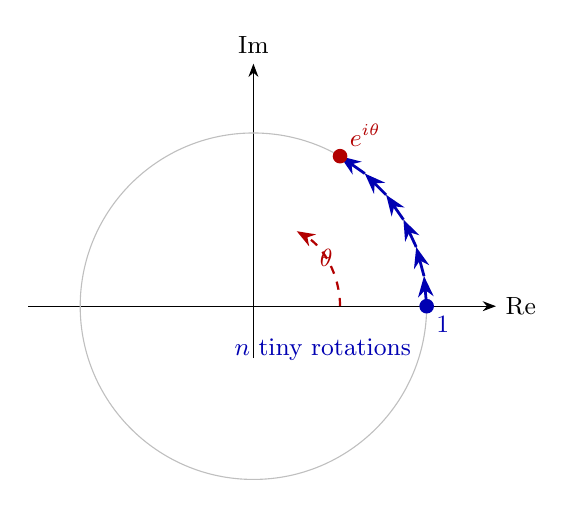
\begin{tikzpicture}[>=Stealth, scale=2.2]
  % axes
  \draw[->] (-1.3,0) -- (1.4,0) node[right] {\small Re};
  \draw[->] (0,-0.3) -- (0,1.4) node[above] {\small Im};
  % unit circle
  \draw[gray!50, thin] (0,0) circle (1);

  % n=6 polygon approximation (θ = π/3 = 60°)
  \def\thetadeg{60}
  \def\nsteps{6}
  \pgfmathsetmacro{\dtheta}{\thetadeg/\nsteps}

  % draw steps
  \foreach \k [evaluate=\k as \angle using \k*\dtheta] in {0,...,\numexpr\nsteps-1} {
    \pgfmathsetmacro{\nextangle}{(\k+1)*\dtheta}
    \draw[->, blue!70!black, line width=1pt]
      ({cos(\angle)},{sin(\angle)}) -- ({cos(\nextangle)},{sin(\nextangle)});
  }

  % start and end points
  \fill[blue!70!black] (1,0) circle (1.2pt) node[below right] {\small $1$};
  \fill[red!70!black] ({cos(\thetadeg)},{sin(\thetadeg)}) circle (1.2pt)
    node[above right] {\small $e^{i\theta}$};

  % arc showing total angle
  \draw[->, red!70!black, thick, dashed] (0.5,0) arc[start angle=0, end angle=\thetadeg, radius=0.5];
  \node[red!70!black] at (0.42,0.28) {\small $\theta$};

  % label
  \node[blue!70!black, font=\small] at (0.4,-0.25) {$n$ tiny rotations};
\end{tikzpicture}
\end{center}

\vfill

Multiply $n$ factors of $\left(1+\frac{i\theta}{n}\right)$:

\begin{itemize}
\item Each rotates by $\approx \theta/n$
\item Total rotation $= n \times \frac{\theta}{n} = \theta$
\item Total stretching $\approx 1$ (modulus stays $\approx 1$)
\end{itemize}

\vfill

\x{Result:} $e^{i\theta}$ is the point on the unit circle at angle $\theta$.

\end{frame}


\begin{frame}[shrink=3]{Geometric Proof: Why It Must Be a Circle}

Consider $y(t) = e^{it}$ as a moving particle. Its position at time $0$ is $y(0) = 1$.

\vfill

The differential equation $y' = iy$ tells us:
\begin{itemize}
\item \x{Velocity} $= i \times$ position
\item Multiplying by $i$ = rotating by $90^\circ$ (from L17)
\end{itemize}

\vfill\pause

So the velocity is always \x{perpendicular} to the position vector!

\vfill

\begin{center}
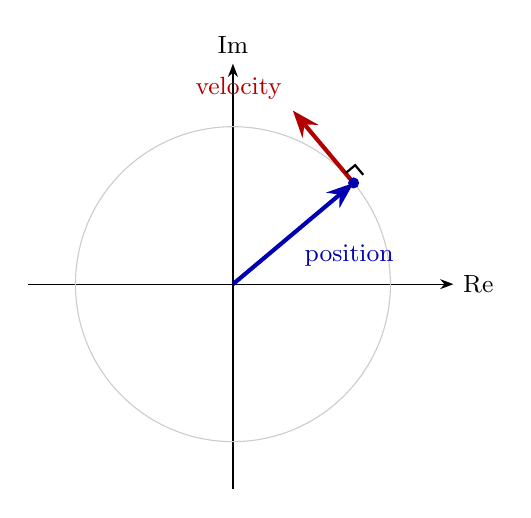
\begin{tikzpicture}[>=Stealth, scale=2.0]
  \draw[->] (-1.3,0) -- (1.4,0) node[right] {\small Re};
  \draw[->] (0,-1.3) -- (0,1.4) node[above] {\small Im};
  \draw[gray!40, thin] (0,0) circle (1);
  % position vector at angle 40°
  \draw[->, blue!70!black, line width=1.5pt] (0,0) -- ({cos(40)},{sin(40)})
    node[midway, below right] {\small position};
  % velocity vector (perpendicular, same length)
  \draw[->, red!70!black, line width=1.5pt] ({cos(40)},{sin(40)}) -- ({cos(40)-0.6*sin(40)},{sin(40)+0.6*cos(40)})
    node[above left] {\small velocity};
  % right angle mark
  \draw[thick] ({cos(40)+0.08*cos(40)},{sin(40)+0.08*sin(40)}) --
    ({cos(40)+0.08*cos(40)-0.08*sin(40)},{sin(40)+0.08*sin(40)+0.08*cos(40)}) --
    ({cos(40)-0.08*sin(40)},{sin(40)+0.08*cos(40)});
  \fill[blue!70!black] ({cos(40)},{sin(40)}) circle (1pt);
\end{tikzpicture}
\end{center}

\end{frame}


\begin{frame}[shrink=3]{The Circle Argument}

Velocity perpendicular to position means:

\vfill

\begin{enumerate}
\item The \x{distance from origin never changes}: if you're always moving sideways, you never get closer or farther. So $|e^{it}| = |e^{i\cdot 0}| = 1$ for all $t$.

\vfill\pause

\item The \x{speed equals the distance} $= 1$ (constant). So the particle moves at constant speed on the unit circle.

\vfill\pause

\item Starting at $1$ (angle $0$), moving at speed $1$ on a circle of circumference $2\pi$: after time $\theta$, the particle has swept angle $\theta$.
\end{enumerate}

\vfill\pause

\begin{block}{Euler's Formula (Geometric Proof)}
$$\boxed{e^{i\theta} = \cos\theta + i\sin\theta}$$
\end{block}

$e^{i\theta}$ is the point on the unit circle at angle $\theta$. That's it.

\end{frame}


\begin{frame}{Euler's Formula from the Power Series (Second Proof)}

For those who know the Taylor series of $\sin$ and $\cos$:

\vfill

Substitute $x = i\theta$ into $e^x = 1 + x + \frac{x^2}{2!} + \cdots$\,:

$$e^{i\theta} = 1 + i\theta + \frac{(i\theta)^2}{2!} + \frac{(i\theta)^3}{3!} + \frac{(i\theta)^4}{4!} + \cdots$$

\vfill\pause

Use $i^2 = -1$, \; $i^3 = -i$, \; $i^4 = 1$, \; $\ldots$ \;:

$$e^{i\theta} = \underbrace{\left(1 - \frac{\theta^2}{2!} + \frac{\theta^4}{4!} - \cdots\right)}_{\cos\theta} + \; i\underbrace{\left(\theta - \frac{\theta^3}{3!} + \frac{\theta^5}{5!} - \cdots\right)}_{\sin\theta}$$

\vfill\pause

Same result. But note: this proof \x{assumes} you already know what $\cos\theta$ and $\sin\theta$ expand to. The geometric proof derives Euler's formula from first principles.

\end{frame}


\begin{frame}{The Geometry of $e^{i\theta}$}

\begin{center}
\begin{tikzpicture}[>=Stealth, scale=2.5]
  % axes
  \draw[->] (-1.4,0) -- (1.5,0) node[right] {\small Re};
  \draw[->] (0,-1.4) -- (0,1.5) node[above] {\small Im};
  % unit circle
  \draw[gray!40, thin] (0,0) circle (1);

  % angle θ ≈ 50°
  \def\mytheta{50}

  % point on circle
  \fill[red!70!black] ({cos(\mytheta)},{sin(\mytheta)}) circle (1.2pt);
  \draw[red!70!black, thick] (0,0) -- ({cos(\mytheta)},{sin(\mytheta)})
    node[above right] {\small $e^{i\theta} = \cos\theta + i\sin\theta$};

  % projections
  \draw[blue!70!black, dashed] ({cos(\mytheta)},{sin(\mytheta)}) -- ({cos(\mytheta)},0)
    node[below] {\small $\cos\theta$};
  \draw[green!60!black, dashed] ({cos(\mytheta)},{sin(\mytheta)}) -- (0,{sin(\mytheta)})
    node[left] {\small $\sin\theta$};

  % angle arc
  \draw[->, thick] (0.35,0) arc[start angle=0, end angle=\mytheta, radius=0.35];
  \node at (0.3,0.15) {\small $\theta$};

  % special points
  \fill (1,0) circle (0.8pt) node[below right] {\small $1$};
  \fill (0,1) circle (0.8pt) node[above left] {\small $i$};
  \fill (-1,0) circle (0.8pt) node[below left] {\small $-1$};
\end{tikzpicture}
\end{center}

\vfill

Special cases:
$$e^{i\pi} = -1, \qquad e^{i\pi/2} = i, \qquad e^{2\pi i} = 1$$

\vfill\pause

General complex exponential: $e^{a+bi} = e^a \cdot e^{bi} = e^a(\cos b + i\sin b)$

\begin{itemize}
\item Real part $a$: controls \x{growth/decay}
\item Imaginary part $b$: controls \x{rotation}
\end{itemize}

\end{frame}


% ┌─────────────────────────────────────────────────────────────────────┐
% │ SECTION 5: EXPONENTIAL OF d/dx IS TAYLOR'S THEOREM                 │
% │                                                                    │
% │ THE MACRO DESIGN: THE PHILOSOPHICAL CLIMAX                        │
% │                                                                    │
% │ This is the deepest insight of the lecture. Taylor's theorem is    │
% │ usually presented as a "approximation" result. Here we reveal      │
% │ its TRUE identity: it is the binomial expansion of                 │
% │ (I + (1/n)(d/dx))^n.                                              │
% │                                                                    │
% │ The key geometric step: for a LINEAR function, adding (1/n)f'(x)  │
% │ shifts the graph left by 1/n. For any smooth function on a tiny    │
% │ interval, it's approximately linear. So the operator               │
% │ I + (1/n)(d/dx) is approximately "shift left by 1/n". Apply n    │
% │ times: shift left by 1.                                            │
% │                                                                    │
% │ This is the "fucking philosophy" — the derivative IS an            │
% │ infinitesimal shift, and exponentiating it gives a finite shift.   │
% └─────────────────────────────────────────────────────────────────────┘
\section{Exponential of $\frac{d}{dx}$ and Taylor's Theorem}


\begin{frame}{What If We Exponentiate a Derivative?}

We defined $e^x = \lim_{n\to\infty}\left(1+\frac{x}{n}\right)^n$ for numbers.

\vfill

\textbf{Bold idea:} Replace $x$ with the operator $\frac{d}{dx}$\,:

$$\exp\!\left(\frac{d}{dx}\right) := \lim_{n\to\infty}\left(I + \frac{1}{n}\frac{d}{dx}\right)^n$$

\vfill\pause

\textbf{Question:} What does this operator \x{do} to a function $f(x)$?

\vfill

Strategy: understand what $\left(I + \frac{1}{n}\frac{d}{dx}\right)$ does, then apply it $n$ times.

\end{frame}


\begin{frame}[shrink=3]{The Operator $I + \frac{1}{n}\frac{d}{dx}$}

This operator maps:
$$f(x) \;\longmapsto\; f(x) + \frac{1}{n}f'(x)$$

\vfill\pause

\textbf{Try a linear function:} $f(x) = kx + b$.

$$f(x) + \frac{1}{n}f'(x) = kx + b + \frac{k}{n} = k\!\left(x + \frac{1}{n}\right) + b = f\!\left(x + \frac{1}{n}\right)$$

\vfill\pause

\begin{center}
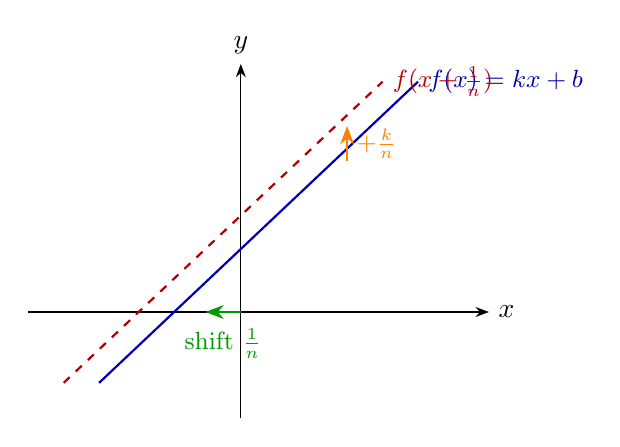
\begin{tikzpicture}[>=Stealth, scale=0.9]
  \draw[->] (-3,0) -- (3.5,0) node[right] {$x$};
  \draw[->] (0,-1.5) -- (0,3.5) node[above] {$y$};
  % original line
  \draw[blue!70!black, thick] (-2,-1) -- (2.5,3.25) node[right] {\small $f(x) = kx+b$};
  % shifted line
  \draw[red!70!black, thick, dashed] (-2.5,-1) -- (2,3.25) node[right] {\small $f(x+\frac{1}{n})$};
  % arrows showing shift
  \draw[<-, thick, green!60!black] (-0.5,0) -- (0,0);
  \node[green!60!black, below] at (-0.25,-0.1) {\small shift $\frac{1}{n}$};
  % arrow showing vertical
  \draw[->, thick, orange] (1.5,2.125) -- (1.5,2.625);
  \node[orange, right] at (1.5,2.375) {\small $+\frac{k}{n}$};
\end{tikzpicture}
\end{center}

\vfill

For a line: shifting \x{up} by $\frac{k}{n}$ $=$ shifting \x{left} by $\frac{1}{n}$.

\end{frame}


\begin{frame}[shrink=3]{Any Smooth Function: Shift Up $\approx$ Shift Left}

On a tiny interval, any smooth function is approximately linear. So the same logic applies:

$$f(x) + \frac{1}{n}f'(x) \;\approx\; f\!\left(x + \frac{1}{n}\right)$$

\vfill

\begin{center}
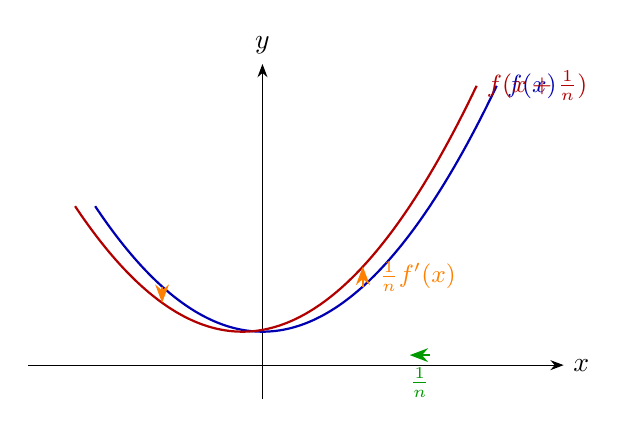
\begin{tikzpicture}[>=Stealth, scale=0.85]
  \draw[->] (-3.5,0) -- (4.5,0) node[right] {$x$};
  \draw[->] (0,-0.5) -- (0,4.5) node[above] {$y$};
  % original parabola
  \draw[blue!70!black, thick, domain=-2.5:3.5, smooth, samples=60]
    plot (\x, {0.3*\x*\x + 0.5}) node[right] {\small $f(x)$};
  % shifted parabola (shifted LEFT by 0.3 ≈ 1/n)
  \draw[red!70!black, thick, domain=-2.8:3.2, smooth, samples=60]
    plot (\x, {0.3*(\x+0.3)*(\x+0.3) + 0.5}) node[right] {\small $f(x+\frac{1}{n})$};
  % arrows showing the vertical difference ≈ derivative
  \draw[->, orange, thick] (1.5, {0.3*1.5*1.5+0.5}) -- (1.5, {0.3*1.8*1.8+0.5});
  \node[orange, right] at (1.6, {0.3*1.5*1.5+0.65}) {\small $\frac{1}{n}f'(x)$};
  \draw[->, orange, thick] (-1.5, {0.3*1.5*1.5+0.5}) -- (-1.5, {0.3*1.2*1.2+0.5});
  % horizontal shift arrow
  \draw[<-, green!60!black, thick] (2.2,0.15) -- (2.5,0.15);
  \node[green!60!black, below] at (2.35, 0.1) {\small $\frac{1}{n}$};
\end{tikzpicture}
\end{center}

\vfill\pause

Adding $\frac{1}{n}f'(x)$ shifts the graph \x{up} by a slope-dependent amount --- which is the same as shifting \x{left} by $\frac{1}{n}$.

\vfill

The operator $I + \frac{1}{n}\frac{d}{dx}$ is approximately \x{``shift left by $\frac{1}{n}$''}.

\end{frame}


\begin{frame}{Apply $n$ Times}

Each application shifts by $\frac{1}{n}$. Apply $n$ times:

\vfill

$$f(x) \;\longrightarrow\; f\!\left(x+\frac{1}{n}\right) \;\longrightarrow\; f\!\left(x+\frac{2}{n}\right) \;\longrightarrow\; \cdots \;\longrightarrow\; f(x+1)$$

\vfill\pause

\begin{block}{The Shift Operator}
$$\boxed{\exp\!\left(\frac{d}{dx}\right)[f](x) = f(x+1)}$$
\end{block}

\vfill

The exponential of the derivative \x{is} the shift-by-one operator!

\vfill\pause

More generally: $\exp\!\left(s\,\frac{d}{dx}\right)[f](x) = f(x+s)$ for any $s$.

\end{frame}


\begin{frame}{Taylor's Theorem IS the Binomial Expansion}

Now use the power series for the exponential:

$$e^{d/dx} = I + \frac{d}{dx} + \frac{1}{2!}\frac{d^2}{dx^2} + \frac{1}{3!}\frac{d^3}{dx^3} + \cdots$$

\vfill\pause

Apply to $f$:

$$\underbrace{e^{d/dx}[f](x)}_{= \; f(x+1)} = f(x) + f'(x) + \frac{f''(x)}{2!} + \frac{f'''(x)}{3!} + \cdots$$

\vfill\pause

\begin{block}{Taylor's Theorem}
$$\boxed{f(x+s) = f(x) + s\,f'(x) + \frac{s^2}{2!}\,f''(x) + \frac{s^3}{3!}\,f'''(x) + \cdots}$$
\end{block}

\vfill

\x{Taylor expansion is nothing more than the binomial expansion applied to the derivative operator.}

\end{frame}


\begin{frame}{Exercise}

\textbf{Exercise.} Using the operator $\exp\!\left(s\,\frac{d}{dx}\right)$, deduce the formula for $f(x+s)$ for general $s$.

\vfill\pause

\textbf{Hint:} Replace $\frac{d}{dx}$ by $s\frac{d}{dx}$ in the limit definition:

$$\exp\!\left(s\,\frac{d}{dx}\right) = \lim_{n\to\infty}\left(I + \frac{s}{n}\frac{d}{dx}\right)^n$$

Each application shifts by $\frac{s}{n}$. After $n$ applications: total shift $= s$.

\end{frame}


% ┌─────────────────────────────────────────────────────────────────────┐
% │ SECTION 6: MATRIX EXPONENTIAL                                      │
% │                                                                    │
% │ THE MACRO DESIGN: THE PAYOFF OF L14–L17                           │
% │                                                                    │
% │ This is the culmination. The same discrete-step trick from §3      │
% │ works for vectors: y'=Ay → y(s) = (I+A/n)^{ns} y(0) → e^{As}    │
% │ y(0). The spectral formula from L15 lets us compute (I+A/n)^{ns}  │
% │ by replacing A with eigenvalues. As n→∞, each                     │
% │ (1+λ_i/n)^{ns} → e^{λ_i s}. This is the payoff: everything      │
% │ students built in L14-L17 makes matrix exponentials computable.    │
% │                                                                    │
% │ The geometric interpretation via eigenspace decomposition shows    │
% │ each eigenspace component evolves independently at rate e^{λ_i s}. │
% └─────────────────────────────────────────────────────────────────────┘
\section{Matrix Exponential}


\begin{frame}{Systems of Differential Equations}

What if the speed of \x{each} quantity depends on \x{all} quantities?

\vfill

$$\mathbf{y}' = A\mathbf{y}, \qquad A = \begin{pmatrix} 0 & -1 \\ 2 & 3 \end{pmatrix}$$

\vfill\pause

Written out:
$$\begin{pmatrix} y_1' \\ y_2' \end{pmatrix} = \begin{pmatrix} 0 & -1 \\ 2 & 3 \end{pmatrix}\begin{pmatrix} y_1 \\ y_2 \end{pmatrix}$$

\vfill

\begin{align*}
y_1' &= -y_2 \\
y_2' &= 2y_1 + 3y_2
\end{align*}

\vfill

The speeds are \x{coupled} --- we cannot solve them separately.

\end{frame}


\begin{frame}{Same Discrete Trick, Matrix Version}

Tiny time step $\frac{1}{n}$:

$$\mathbf{y}\!\left(\frac{1}{n}\right) \;\approx\; \mathbf{y}(0) + \frac{1}{n}\,A\,\mathbf{y}(0) \;=\; \left(I + \frac{A}{n}\right)\mathbf{y}(0)$$

\vfill\pause

After $n$ steps:

$$\mathbf{y}(1) \;=\; \left(I + \frac{A}{n}\right)^n \mathbf{y}(0)$$

\vfill\pause

After $ns$ steps (reaching time $s$):

$$\mathbf{y}(s) \;=\; \left(I + \frac{A}{n}\right)^{ns} \mathbf{y}(0)$$

\end{frame}


\begin{frame}{Definition of Matrix Exponential}

As $n \to \infty$:

\begin{block}{Definition}
$$e^{A} \;:=\; \lim_{n\to\infty}\left(I + \frac{A}{n}\right)^n$$
\end{block}

\vfill

Same definition as before --- replace the number $x$ with a matrix $A$, and $1$ with $I$.

\vfill\pause

\begin{block}{Solution}
The system $\mathbf{y}' = A\mathbf{y}$, \; $\mathbf{y}(0) = \mathbf{y}_0$ has solution:
$$\boxed{\mathbf{y}(s) = e^{As}\,\mathbf{y}(0)}$$
\end{block}

\vfill\pause

\textbf{But how do we compute $e^{As}$?}

\end{frame}


\begin{frame}{The Spectral Formula --- The Payoff}

From L15: the \x{spectral formula} says that for any polynomial $g$,

$$g(A) = g(\lambda_1)\,P_1 + g(\lambda_2)\,P_2$$

\vfill\pause

The key observation: $\left(I+\frac{A}{n}\right)^{ns}$ is a \x{polynomial} in $A$ (for each finite $n$).

\vfill

So by the spectral formula:

$$\left(I+\frac{A}{n}\right)^{ns} = \left(1+\frac{\lambda_1}{n}\right)^{ns} P_1 + \left(1+\frac{\lambda_2}{n}\right)^{ns} P_2$$

\vfill\pause

As $n \to \infty$: each $\left(1+\frac{\lambda_i}{n}\right)^{ns} \to e^{\lambda_i s}$.

\vfill

\begin{block}{Matrix Exponential via Spectral Decomposition}
$$\boxed{e^{As} = e^{\lambda_1 s}\,P_1 + e^{\lambda_2 s}\,P_2}$$
\end{block}

\end{frame}


\begin{frame}[shrink=3]{Concrete Calculation}

$A = \begin{pmatrix}0&-1\\2&3\end{pmatrix}$, \; $\det(tI - A) = (t-1)(t-2)$. \; Eigenvalues: $\lambda_1 = 1$, $\lambda_2 = 2$.

\vfill\pause

Spectral projections (from L15):

$$P_1 = \frac{A-2I}{1-2} = \begin{pmatrix}2&1\\-2&-1\end{pmatrix}, \qquad P_2 = \frac{A-I}{2-1} = \begin{pmatrix}-1&-1\\2&2\end{pmatrix}$$

\vfill\pause

Matrix exponential:

$$e^{As} = e^{s}\begin{pmatrix}2&1\\-2&-1\end{pmatrix} + e^{2s}\begin{pmatrix}-1&-1\\2&2\end{pmatrix}$$

\vfill\pause

Solution:
$$\begin{pmatrix}y_1(s)\\y_2(s)\end{pmatrix} = e^{As}\begin{pmatrix}y_1(0)\\y_2(0)\end{pmatrix} = \begin{pmatrix}(2e^s - e^{2s})\,y_1(0) + (e^s - e^{2s})\,y_2(0) \\ (-2e^s + 2e^{2s})\,y_1(0) + (-e^s + 2e^{2s})\,y_2(0)\end{pmatrix}$$

\end{frame}


\begin{frame}{Geometric Understanding via Eigenspaces}

Decompose the initial condition using the spectral projections:

$$\mathbf{y}(0) = P_1\,\mathbf{y}(0) + P_2\,\mathbf{y}(0) = \mathbf{w}(0) + \mathbf{u}(0)$$

\vfill\pause

Each piece lives in an eigenspace, so each evolves \x{independently}:

\vfill

\begin{align*}
\mathbf{w}' &= A\mathbf{w} = 1 \cdot \mathbf{w} &&\implies \mathbf{w}(s) = e^{s}\,\mathbf{w}(0) \\[6pt]
\mathbf{u}' &= A\mathbf{u} = 2 \cdot \mathbf{u} &&\implies \mathbf{u}(s) = e^{2s}\,\mathbf{u}(0)
\end{align*}

\vfill\pause

Total:
$$\mathbf{y}(s) = e^s\,\mathbf{w}(0) + e^{2s}\,\mathbf{u}(0)$$

\vfill

Each eigenspace component grows at its own rate. The \x{larger eigenvalue dominates} as $s \to \infty$.

\end{frame}


% ┌─────────────────────────────────────────────────────────────────────┐
% │ SECTION 7: COMPLEX EIGENVALUES — ROTATION                          │
% │                                                                    │
% │ THE MACRO DESIGN: L17 MEETS EULER'S FORMULA                       │
% │                                                                    │
% │ In L17 we found that the rotation matrix has eigenvalues ±i.       │
% │ Now we can compute e^{Rθ} using the spectral formula + Euler.     │
% │ The result: the rotation matrix by angle θ. Complex eigenvalues   │
% │ = oscillation/rotation, real eigenvalues = growth/decay.           │
% └─────────────────────────────────────────────────────────────────────┘
\section{Complex Eigenvalues}


\begin{frame}{What If Eigenvalues Are Complex?}

From L17: the \x{rotation matrix} $R = \begin{pmatrix}0&-1\\1&0\end{pmatrix}$ has eigenvalues $\lambda = \pm i$.

\vfill\pause

The spectral formula still works over $\mathbb{C}$:

$$e^{R\theta} = e^{i\theta}\,P_1 + e^{-i\theta}\,P_2$$

\vfill\pause

Using Euler's formula:
\begin{itemize}
\item $e^{i\theta} = \cos\theta + i\sin\theta$
\item $e^{-i\theta} = \cos\theta - i\sin\theta$
\end{itemize}

\end{frame}


\begin{frame}{Computing the Projections}

Eigenvalues: $\lambda_1 = i$, $\lambda_2 = -i$.

\vfill

$$P_1 = \frac{R - (-i)I}{i - (-i)} = \frac{R + iI}{2i}$$

\vfill\pause

$$= \frac{1}{2i}\begin{pmatrix}i & -1 \\ 1 & i\end{pmatrix} = \frac{1}{2}\begin{pmatrix}1 & i \\ -i & 1\end{pmatrix}$$

\vfill\pause

Similarly: $P_2 = \dfrac{R - iI}{-2i} = \dfrac{1}{2}\begin{pmatrix}1 & -i \\ i & 1\end{pmatrix}$

\vfill

Note: $P_2 = \overline{P_1}$ --- conjugate pair of projections for conjugate pair of eigenvalues (the symmetry principle from L17!).

\end{frame}


\begin{frame}{The Result: Rotation by Any Angle}

\vspace{-2mm}
$$e^{R\theta} = e^{i\theta}\cdot\frac{1}{2}\begin{pmatrix}1&i\\-i&1\end{pmatrix} + e^{-i\theta}\cdot\frac{1}{2}\begin{pmatrix}1&-i\\i&1\end{pmatrix}$$

\vfill\pause

Look at the $(1,1)$ entry: $\;\frac{1}{2}(e^{i\theta} + e^{-i\theta}) = \cos\theta$

Look at the $(2,1)$ entry: $\;\frac{1}{2}(-i\,e^{i\theta} + i\,e^{-i\theta}) = \frac{i(e^{-i\theta}-e^{i\theta})}{2} = \sin\theta$

\vfill\pause

Collecting all entries:

\begin{block}{Rotation Matrix}
$$\boxed{e^{R\theta} = \begin{pmatrix}\cos\theta & -\sin\theta \\ \sin\theta & \cos\theta\end{pmatrix}}$$
\end{block}

\vfill

The matrix exponential of the $90^\circ$ rotation generator gives \x{rotation by any angle $\theta$}.

\end{frame}


\begin{frame}{The Big Picture: Real vs.\ Complex Eigenvalues}

\begin{center}
\renewcommand{\arraystretch}{1.8}
{\small
\begin{tabular}{c|c|c}
\textbf{Eigenvalue} & \textbf{$e^{\lambda s}$} & \textbf{Meaning} \\
\hline
$\lambda > 0$ & grows & Exponential \x{growth} \\
$\lambda < 0$ & decays & Exponential \x{decay} \\
$\lambda = i\omega$ & rotates & Pure \x{oscillation} \\
$\lambda = a + bi$ & $e^{as} \cdot e^{ibs}$ & Growth/decay $\times$ oscillation \\
\end{tabular}
}
\end{center}

\vfill\pause

\x{Real eigenvalues produce growth or decay.}

\x{Complex eigenvalues produce rotation and oscillation.}

\vfill

The spectral formula $e^{As} = \sum e^{\lambda_i s}\,P_i$ handles \x{all cases uniformly}.

\end{frame}


% ┌─────────────────────────────────────────────────────────────────────┐
% │ SUMMARY                                                             │
% └─────────────────────────────────────────────────────────────────────┘
\section{Summary}


\begin{frame}{One Definition, Four Faces}

\begin{block}{The Definition}
$$e^X = \lim_{n\to\infty}\left(I + \frac{X}{n}\right)^n$$
\end{block}

\vfill

\begin{center}
\renewcommand{\arraystretch}{1.6}
\begin{tabular}{c|c|c}
$X$ & $e^X$ & Meaning \\
\hline
$x \in \mathbb{R}$ & $e^x$ & Growth / decay \\
$i\theta$ & $\cos\theta + i\sin\theta$ & Rotation (Euler) \\
$A$ (matrix) & $\sum e^{\lambda_i s} P_i$ & Solve $\mathbf{y}' = A\mathbf{y}$ \\
$\frac{d}{dx}$ & Shift operator & Taylor's theorem
\end{tabular}
\end{center}

\vfill\pause

\x{Repeated tiny nudges compound into a smooth transformation.}

\vfill

The binomial expansion of the limit gives the power series. Everything is one idea.

\end{frame}


\end{document}
